\documentclass{sig-alternate-05-2015}

\usepackage{amsmath}
\usepackage{graphicx}
\usepackage{listings}
\usepackage{microtype}
\usepackage{pslatex}
\usepackage{relsize}
\usepackage[pageanchor=false]{hyperref}

% Add page numbers, remove copyright box.  For submitted version only.
\pagenumbering{arabic}
\makeatletter
\def\@copyrightspace{\relax}
\makeatother

% At least 80% of every float page must be taken up by
% floats; there will be no page with more than 20% white space.
\def\topfraction{.8}
\def\dbltopfraction{\topfraction}
\def\floatpagefraction{\topfraction}     % default .5
\def\dblfloatpagefraction{\topfraction}  % default .5
\def\textfraction{.2}


% I copied some formatting settings from another template I have used for homework in the past, but I don't like
% how it does comments and will change the formatting.
\lstset{
    language=Java,
    basicstyle=\sf\footnotesize,
    aboveskip={1.0\baselineskip},
    belowskip={1.0\baselineskip},
    columns=fixed,
    extendedchars=true,
    breaklines=true,
    tabsize=4,
    prebreak=\raisebox{0ex}[0ex][0ex]{\ensuremath{\hookleftarrow}},
    showtabs=false,
    showspaces=false,
    showstringspaces=false,
    numberstyle=\small,
    stepnumber=1,
    numbersep=10pt,
    captionpos=b,
    escapeinside={\%*}{*)}
}

% \|name| or \mathid{name} denotes identifiers and slots in formulas
\def\|#1|{\mathid{#1}}
\newcommand{\mathid}[1]{\ensuremath{\mathit{#1}}}
% \<name> or \codeid{name} denotes computer code identifiers
\def\<#1>{\codeid{#1}}
\protected\def\codeid#1{\ifmmode{\mbox{\sf{#1}}}\else{\sf #1}\fi}


\begin{document}

\special{papersize=8.5in,11in}
\setlength{\pdfpageheight}{\paperheight}
\setlength{\pdfpagewidth}{\paperwidth}

\title{Preventing Signedness Errors in Numerical Computations}

\numberofauthors{1} %  in this sample file, there are a *total*
\author{
Christopher A. Mackie\\
       \affaddr{University of Washington Computer Science \& Engineering}\\
       \affaddr{Seattle, WA, USA}\\
       \email{mackic@cs.washington.edu}
}

\maketitle

\section{Problem and Motivation}

A signed integer uses the first bit of the machine representation to
represent the sign (positive or negative).  An unsigned integer uses all
bits of the machine representation to represent the value.
An unsigned integer can represent a larger range of positive numbers, but
cannot represent negative numbers.
Unsigned integers are useful, so many programming languages support them;
for example, Java 8 provides utility methods for unsigned
integers~\cite{JDK8UnsignedIntegerArithmetic2012}.  However, unsigned
integers are also error-prone:  using an unsigned integer where a signed
one is expected, or performing certain arithmetic operations and
comparisons on unsigned integers, can lead to unexpected results.

We call an operator ``insensitive'' if it produces a correct signed result
when run on two signed values, and it produces a correct unsigned result
when run on two unsigned values.  We call an operator ``sensitive'' if it
produces incorrect results when run on two unsigned values.  For such
operations, a programmer must run a different operator depending on whether
the operands are signed or unsigned.  See Figure~\ref{fig:operators} for
an example of insensitive and sensitive operators.

Misuse of unsigned values can be categorized as follows:

\begin{itemize}\itemsep 0pt \parskip 0pt
  \item Using a sensitive operator or routine with operands of opposite signedness to the implementation of the operator.
  \item Mixing signed and unsigned arguments to any operator, sensitive or insensitive.
\end{itemize}

The first line of defense against most bugs is the compiler. When the
compiler is unable to catch bugs it falls on the programmer to identify and
eliminate them, which is prone to human error. The compiler 
is not helpful in finding bugs related to using unsigned
numbers, because Java's unsigned
integers are supported by a library rather than built into Java.


\section{Approach and Uniqueness}

Our approach to detecting and preventing signedness errors is to use a type
system. This has a number of benefits.
%
Compile-time checking permits developers
to catch bugs before they become problems for their end-users.
%
Type systems are a familiar to programmers, who understand how to use them
and how to interpret their warning messages.
%
Type-checking is modular and fast.

% Figure appears late in the LaTeX file to prevent it from being placed in
% the first column of the paper.
\begin{figure}
\begin{lstlisting}
byte x = 255;
byte y = 254;

byte sub = x - y;
// Result is 1, which is correct when:
//  * x, y, and sub are signed.
//  * x, y, and sub are unsigned.

byte div = y / x;
// Result is 2.
//  * Correct for signed x, y, and div.
//  * Incorrect for unsigned x, y, and div.
\end{lstlisting}
\vspace{-10pt}
\caption{Subtraction is an insensitive operator, and
  division is a sensitive operator.}
\label{fig:operators}
\end{figure}


\begin{figure}
    \centering
    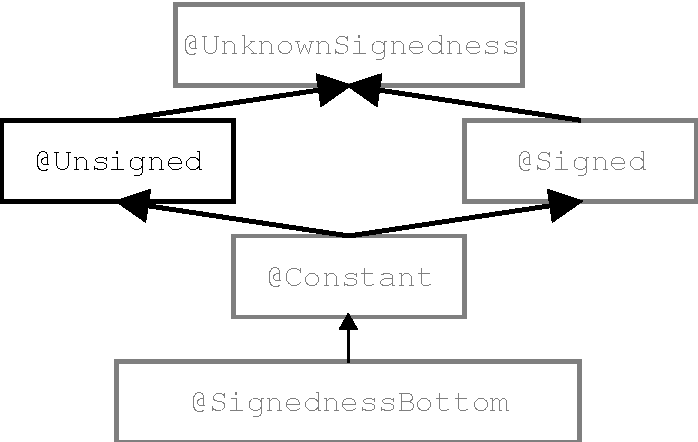
\includegraphics[width=0.4\textwidth]{signedness}
    \caption{The type qualifier hierarchy of the signedness annotations.
The default annotation is \<@Signed>.
Qualifiers in gray are used internally by the type system and need not be
written by a programmer.}
    \label{fig:my_label}
\end{figure}

We have defined a signedness type system with 5 type qualifiers:

\begin{itemize}\itemsep 0pt \parskip 0pt
  \item The Unsigned type is the only user defined type. This is the only way it can be introduced into a program. This type signifies that a value is unsigned, that it is not to be put into any situation in which Java's default assumption of signed integers may place the program into a bad state.
  \item The Signed type is similarly meant for signed integers, which Java is free to interpret as it pleases. With the exception of logical right shifts, no operator restrictions are placed on Signed values by the Signedness Checker.
  \item The Constant type is for values which are known at compile time, and could potentially be signed or unsigned depending on how the programmer intends to use them. Even negative literals may be used as a convenience placeholder for a large positive unsigned integer, so we say a constant value is both signed and unsigned.
  \item The UnknownSignedness type is for values which are either outside of the Signedness Checker's scope, or have been mixed so that the Signedness Checker no longer knows what signedness to assign to them. In the second case, the presence of an UnknownSignedness value almost always indicates an issue.
  \item The SignednessBottom type is never assigned to anything, and if this type is present in an AST, there is an issue.
\end{itemize}

Furthermore, the type system prevents the third class of unsigned integer bugs, the interchange of signed and unsigned integers, by the nature of its hierarchy, shown in Figure~\ref{fig:my_label}.

Types are introduced into a program either by the user, for Unsigned values, or by the the Signedness Checker using its type introduction rules. Types are introduced as follows, noting that these checks are done in a defined order:

\begin{enumerate}\itemsep 0pt \parskip 0pt
  \item If a user has declared an expression to be Unsigned, then it is assigned this type.
  \item If an expression is not a leaf in the syntax tree (i.e. not a terminating symbol), its type is the least upper bound of the types in the tree rooted on it.
  \item If an expression is a constant at compile time, it is given the Constant type.
  \item If an expression is an integral type, for which signedness must be considered, it is given the Signed type.
  \item If no other type was assigned to an expression, it's signedness is not known to the Signedness Checker and it is given the top type, UnknownSignedness.
\end{enumerate}

The real work of the Signedness Type System is done by its type rules, which eliminate the first two classes of bugs associated with unsigned integers. Generally speaking, these type rules are as follows:

\begin{itemize}\itemsep 0pt \parskip 0pt
  \item Unsigned values may not be used as input for sensitive operators, as such operators are implemented in Java for signed integers.
  \item With the exception of shifts, no operator may take as input a mix of Signed and Unsigned values.
  \item Logical right shifts may only be applied to Unsigned values.
  \item Arithmetic right shifts may only be applied to Signed values.
\end{itemize}

These rules prevent Unsigned numbers from being used in ways which would allow Java to incorrectly handle them. As ultimately unsigned integers are simply an alternative representation, we are concerned only that the representation is conserved. This means that the signed implementation of an insensitive operator may be used on an Unsigned value because the result is the same as if the unsigned implementation were used.

\section{Background and Implementation}

% I will go over this section later to include citations. Right now I just want to get words on paper.

We seek here to build a verification tool, so that developers may use it to be sure that their software is free of bugs related to unsigned integers. This means that our approach must be sound; that if it says a program is free of bugs it is so. We build our solution on top of the Checker Framework, an API developed by the University of Washington to provide a platform for pluggable type systems to be introduced into a custom version of the javac compiler. This allows our type system to be checked concurrently with that of Java, and potentially other type systems.

The Checker Framework provides the groundwork for many similar type systems solving other common classes of bugs. Such verification tools, called checkers, provide an excellent template to follow when implementing a type system in this framework. We discussed the Signedness Type System, which at a high level consists of a series of qualifiers with some hierarchy, a series of introduction rules for determining expression types, and several type rules for issuing errors for malformed code. These parts are implemented in a checker as follows:

\begin{itemize}\itemsep 0pt \parskip 0pt
  \item Type qualifiers are implemented with type annotations. The Checker Framework provides several helper annotations to allow the structure of the type hierarchy and some introduction rules to be defined declaratively.
  \item More complex introduction rules are used procedurally to determine the type of expression trees in the syntax tree using a type factory.
  \item Type rules are enforced by a visitor which visits each node of the syntax tree to determine if it follows type rules.
\end{itemize}

Like other checkers included in the Checker Framework, such as the Nullness Checker, the Signedness Checker must conform to language specifications outside of its control. This can lead to tough design decisions which in turn may result in false negatives for one design, or false positives for another. Because the Signedness Checker is intended to be a sound tool, its design is always in favor of false negatives over false positives so that if the checker passes a program, that program is free of signedness bugs. This is a similar design strategy in other Checker Framework checkers, which provided us inspiration on how to consider the strength of the type system from a high level. The Signedness Checker is available with the \href{https://github.com/typetools/checker-framework}{Checker Framework}.

\section{Results and Contributions}
% I will go back through this section and cite where needed

To put the Signedness Checker to the test, we used it to analyze jake2, a Java port of the popular '90s video game, Quake II. This case study is a large, complex piece of software, with many instances of unsigned integers being used in system code. Without applying annotations the Signedness Checker listed many perceived errors with using a logical right shift, sometimes called an unsigned right shift, on signed operands. Many of these were eliminated by annotating documented unsigned integers, but a few persisted. By comparing jake2 with the original C implementation, we have been able to identify and record semantic differences between the two systems, particularly in the usage of right shifts. In detail, the jake2 implementation uses logical right shifts on Signed values in many locations where the C implementation used arithmetic right shifts. It is possible that if a negative value passed to such regions of code that the two implementations will behave differently in a way noticible to the end-user. Further analysis is required to determine if these differences indeed have noticeable effects. Furthermore, we have been able to identify one bug, in which an unsigned integer is passed to a utility function which prints its value during debugging. No special handling of the unsigned value is done, so it is printed as if signed, which can possibly lead to erroneous output for values outside signed positive range.

\bibliographystyle{abbrv}
\bibliography{bibstring-unabbrev,ernst,generals,invariants,types}

\end{document}

%  LocalWords:  papersize Signedness Mackie signedness javac's jake2 90s
%  LocalWords:  UnknownSignedness SignednessBottom
